\documentclass[../../main]{subfiles}

\begin{document}
\chapter{数ベクトル空間}
\label{chapter:numerical_vector_space}

\begin{lead}
  \cref{chapter:numerical_vector_space}では,数ベクトル空間における直交性と最良近似の関係を説明する.
\end{lead}

\section{直交射影}

本節では,あるベクトルを他のベクトルの線型結合で近似する手法を説明する.
特に断りのない限り,\cref{chapter:numerical_vector_space}において\(\numset{K}\)は\(\numset{R}\)か\(\numset{C}\)を意味し,
\(\innerp{\holder}{\holder}\)は\(\numset{K}^n\)の標準内積を意味する.また
\[
  \vnorm{\vect{x}} = \sqrt{\innerp{\vect{x}}{\vect{x}}}
  = \sqrt{\abs{x_1}^2+\dots+\abs{x_n}^2}
  \quad\text{(\(\vect{x}=\trps{\inlinevec{x_1 & \cdots & x_n}}\in\numset{K}^n\))}
\]
とする\index{\(\vnorm{\holder}\)}.

\subsection{直交射影}
\(\numset{K}^n\)のベクトル\(\vect{x}\),部分空間\(V\)が与えられたとき,\(V\)の元で\(\vect{x}\)に最も近いベクトル,すなわち,距離\(\vnorm{\vect{x}-\vect{m}}\)を最小にする\(\vect{m}\in V\)について考えよう.

\begin{figure}[htbp]
  \centering
  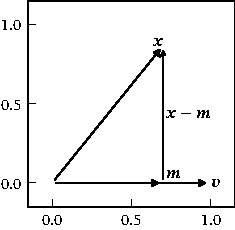
\includegraphics{proj2d.pdf}
  \caption{\(V=\spannedby\Set{\vect{v}}\)の元で\(\vect{x}\)に最も近いベクトル\(\vect{m}\)の様子.}
  \label{figure:proj2d}
\end{figure}

\(\numset{K}^n\)が平面\(\numset{R}^2\)で,\(V\)があるベクトル\(\vect{v}\neq\zvec\)により生成される直線\(\spannedby\Set{\vect{v}}\)の場合について,\(\vect{m}\)を図示したのが\cref{figure:proj2d}である.
\cref{figure:proj2d}を見ると,\(\vect{x}-\vect{m}\)は\(\vect{v}\)と直交しているのが分かる.

一般の部分空間\(V\subset\numset{K}^n\)についても,直交性は最良近似を特徴づける.証明へと入る前に,便利な記法を2つ定義しておく.

\begin{definition}{\(\argmin\),\(\argmax\)}{argmin_argmax}\index{\(\argmin\)}\index{\(\argmax\)}
  \(X\)を集合とする.集合\(S\subset X\)と関数\(f\colon X\to\numset{R}\)に対して,\(S\)の部分集合\(\argmin_{x\in S}f(x)\),\(\argmax_{x\in S}f(x)\)を以下の通り定義する.
  \begin{align*}
    \argmin_{x\in S}f(x) &= \Set{x\in S\given y\in S\implies f(y)\geq f(x)}, \\
    \argmax_{x\in S}f(x) &= \Set{x\in S\given y\in S\implies f(y)\leq f(x)}
  \end{align*}
\end{definition}

\cref{definition:argmin_argmax}からただちに,次のことが分かる.

\begin{proposition}{}{}
  \(S\)の元\(a\)に関する以下の条件は同値であり,同様のことが\(\argmax\)についても成り立つ.
  \begin{enumerate}
    \item \(a\in\argmin_{x\in S}f(x)\)である
    \item 関数\(f\)は\(S\)上で最小値に達して,その値は\(f(a)\)である
  \end{enumerate}
\end{proposition}

\begin{example}
  \(\argmin_{x\in\coival{0}{\infty}}\exp(-x)=\argmax_{x\in\coival{0}{\infty}}\exp(x)=\emptyset\)である.
  また\(\argmin_{x\in\numset{R}}\abs{\sin(x)}=\Set{n\krez\given n\in\numset{Z}}\)である.
\end{example}

\begin{figure}[htbp]
  \centering
  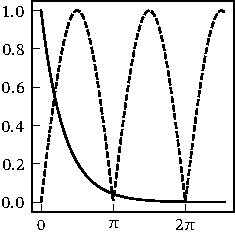
\includegraphics{argmin.pdf}
  \caption{\(\exp(-x)\)と\(\abs{\sin(x)}\)のグラフ.\(\exp(-x)\to 0\)(\(x\to\infty\))であるが,\(\exp(-x)=0\)となる実数\(x\)は存在しないことに注意.}
\end{figure}

\(\numset{K}=\numset{R}\)の場合も同様に証明できるので,\cref{proposition:finite_projection}まで証明では\(\numset{K}=\numset{C}\)を仮定する.また,部分空間が\(\Set{\zvec}\)でないことも仮定する.

\begin{proposition}{}{finite_convex_projection}
  \(\vect{x}\in\numset{K}^n\)かつ,\(V\)は\(\numset{K}^n\)の部分空間とする.
  このとき,\(\argmin_{\vect{y}\in V}\vnorm{\vect{x}-\vect{y}}\)はただ1つの元からなる集合である.
\end{proposition}

\begin{proof}
  \(\basis{B}=\Set{\vect{e}_1,\dots,\vect{e}_m}\)を\(V\)の正規直交基底とすると,
  \(V\)は\(\Set{z_1\vect{e}_1+\dots+z_m\vect{e}_m\given z_1,\dots,z_m\in\numset{C}}\)と書ける.
  したがって,関数\(f(\vect{z})=\vnorm{\vect{x}-(z_1\vect{e}_1+\dots+z_m\vect{e}_m)}\)(\(\vect{z}=\trps{\inlinevec{z_1 & \cdots & z_m}}\in\numset{C}^m\))の最小値が\(\min_{\vect{y}\in V}\vnorm{\vect{x}-\vect{y}}\)である.

  \(\argmin_{\vect{z}\in\numset{C}^m}f(\vect{z})\)を求める.\(\basis{B}\)は正規直交基底だから
  \[
    \vnorm*{\sum_{i=1}^mz_i\vect{e}_i}^2 = \innerp*{\sum_{i=1}^mz_i\vect{e}_i}{\sum_{j=1}^mz_j\vect{e}_j}
    = \sum_{i=1}^m\sum_{j=1}^mz_i\conj{z_j}\innerp{\vect{e}_i}{\vect{e}_j}
    = \sum_{i=1}^m\sum_{j=1}^mz_i\conj{z_j}\kdelta{i}{j}
    = \sum_{i=1}^m\abs{z_i}^2
  \]
  となる.したがって(\(\sum_{k=1}^m\)を\(\sum\)と略記すると)
  \begin{align*}
    f(\vect{z})^2 &= \vnorm*{\vect{x}-\sum z_k\vect{e}_k}^2 = \vnorm{\vect{x}}^2-2\rpart\innerp*{\vect{x}}{\sum z_k\vect{e}_k}+\vnorm*{\sum z_k\vect{e}_k}^2 \\
    &= \vnorm{\vect{x}}^2-2\sum\rpart[\conj{z_k}\innerp{\vect{x}}{\vect{e}_k}]+\sum\abs{z_k}^2
  \end{align*}
  である.よって,\(f(\vect{z})^2\)は\(s_k=\rpart z_k\)と\(t_k=\ipart z_k\)の式で
  \begin{align*}
    f(\vect{z})^2 &= \vnorm{\vect{x}}^2+\sum(-2\rpart[(s_k-\iuni t_k)\innerp{\vect{x}}{\vect{e}_k}]+s_k^2+t_k^2) \\
    &= \vnorm{\vect{x}}^2+\sum(-2(s_k\rpart\innerp{\vect{x}}{\vect{e}_k}+t_k\ipart\innerp{\vect{x}}{\vect{e}_k})+s_k^2+t_k^2) \\
    &= \vnorm{\vect{x}}^2+\sum((s_k-\rpart\innerp{\vect{x}}{\vect{e}_k})^2+(t_k-\ipart\innerp{\vect{x}}{\vect{e}_k})^2-\abs{\innerp{\vect{x}}{\vect{e}_k}}^2)
  \end{align*}
  と書けるので,次式が成立する.
  \begin{equation}
    \label{equation:pre_bessels_inequality}
    f(\vect{z})^2 = \vnorm{\vect{x}}^2+\sum_{k=1}^m\abs{z_k-\innerp{\vect{x}}{\vect{e}_k}}^2-\sum_{k=1}^m\abs{\innerp{\vect{x}}{\vect{e}_k}}^2
  \end{equation}

  \cref{equation:pre_bessels_inequality}より\(\argmin_{\vect{z}\in\numset{C}^m}f(\vect{z})=\Set{\trps{\inlinevec{\innerp{\vect{x}}{\vect{e}_1} & \cdots & \innerp{\vect{x}}{\vect{e}_m}}}}\)であるから,
  \(\argmin_{\vect{y}\in V}\vnorm{\vect{x}-\vect{y}}=\Set{\innerp{\vect{x}}{\vect{e}_1}\vect{e}_1+\dots+\innerp{\vect{x}}{\vect{e}_m}\vect{e}_m}\)である.
\end{proof}

なお,\cref{proposition:finite_convex_projection}は部分空間よりも少し広い対象(閉凸集合)へと一般化できるのだが,そのことは\cref{xr-chapter:hilbert_space}であらためて扱う.

\begin{proposition}{}{weak_finite_projection}
  \(\vect{x}\in\numset{K}^n\)かつ,\(V\)は\(\numset{K}^n\)の部分空間とする.
  \(V\)のある元\(\vect{m}\)が任意の\(\vect{y}\in V\)に対して\(\innerp{\vect{x}-\vect{m}}{\vect{y}}=0\)を満たすとき,
  \(\vect{m}\in\argmin_{\vect{y}\in V}\vnorm{\vect{x}-\vect{y}}\)である.
\end{proposition}

\begin{proof}
  任意の\(\vect{y}\in V\)について,\(\vect{y}-\vect{m}\in V\)だから
  \begin{align*}
    \vnorm{\vect{x}-\vect{y}}^2 &= \vnorm{(\vect{x}-\vect{m})-(\vect{y}-\vect{m})}^2 \\
    &= \vnorm{\vect{x}-\vect{m}}^2-2\rpart\innerp{\vect{x}-\vect{m}}{\vect{y}-\vect{m}}+\vnorm{\vect{y}-\vect{m}}^2 \\
    &= \vnorm{\vect{x}-\vect{m}}^2+\vnorm{\vect{y}-\vect{m}}^2 \geq \vnorm{\vect{x}-\vect{m}}^2
  \end{align*}
  である.よって\(\vnorm{\vect{x}-\vect{m}}=\min_{\vect{y}\in V}\vnorm{\vect{x}-\vect{y}}\)である.
\end{proof}

\cref{proposition:weak_finite_projection}からは,仮定「任意の\(\vect{y}\in V\)に対して\(\innerp{\vect{x}-\vect{m}}{\vect{y}}=0\)」を満たす\(\vect{m}\in V\)が存在するかどうかは分からない.
しかし実は,仮定を満たす\(\vect{m}\)は一意に定まり,それは\(\argmin_{\vect{y}\in V}\vnorm{\vect{x}-\vect{y}}\)のただ1つの元である.

\begin{proposition}{}{finite_projection}
  \(\vect{x}\in\numset{K}^n\)かつ,\(V\)は\(\numset{K}^n\)の部分空間とする.
  このとき,\(V\)の元\(\vect{m}\)に関する以下の条件は同値であり,条件を満たす\(\vect{m}\)はただ1つ存在する.
  \begin{enumerate}
    \item \(\vect{m}\in\argmin_{\vect{y}\in V}\vnorm{\vect{x}-\vect{y}}\)である
    \item 任意の\(\vect{y}\in V\)に対して\(\innerp{\vect{x}-\vect{m}}{\vect{y}}=0\)である
  \end{enumerate}
\end{proposition}

\begin{proof}
  \cref{proposition:finite_convex_projection}より,\(\vect{n}\in\argmin_{\vect{y}\in V}\vnorm{\vect{x}-\vect{y}}\)を満たす\(\vect{n}\in V\)がただ1つ存在する.
  そして\cref{proposition:weak_finite_projection}より,\(\vect{m}\in V\)が任意の\(\vect{y}\in V\)に対して\(\innerp{\vect{x}-\vect{m}}{\vect{y}}=0\)を満たすなら\(\vect{m}=\vect{n}\)である.

  したがって,\(\vect{n}\)がすべての\(\vect{v}\in V\)に対して\(\innerp{\vect{x}-\vect{n}}{\vect{v}}=0\)を満たすことを示せばよい.
  \(\vect{v}\in V\)を任意にとる.\(\vect{v}=\vect{0}\)なら明らかに\(\innerp{\vect{x}-\vect{n}}{\vect{v}}=0\)である.
  \(\vect{v}\neq\vect{0}\)のとき,\(\vect{n}\)の定義から\(t\in\numset{R}\)の関数\(f(t)=\vnorm{\vect{x}-(\vect{n}+t\vect{v})}^2\)は\(t=0\)で最小値をとる.一方
  \begin{align*}
    f(t) &= \vnorm{\vect{x}-\vect{n}-t\vect{v}}^2 = \vnorm{\vect{x}-\vect{n}}^2-2t\rpart\innerp{\vect{x}-\vect{n}}{\vect{v}}+t^2\vnorm{\vect{v}}^2 \\
    &= \pqty*{\vnorm{\vect{v}}t-\frac{\rpart\innerp{\vect{x}-\vect{n}}{\vect{v}}}{\vnorm{\vect{v}}}}^2+\vnorm{\vect{x}-\vect{n}}^2-\pqty*{\frac{\rpart\innerp{\vect{x}-\vect{n}}{\vect{v}}}{\vnorm{\vect{v}}}}^2
  \end{align*}
  は\(t=(\rpart\innerp{\vect{x}-\vect{n}}{\vect{v}})/\vnorm{\vect{v}}^2\)で最小値をとる.よって\(\rpart\innerp{\vect{x}-\vect{n}}{\vect{v}}=0\)である.

  同様に,関数\(g(t)=\vnorm{\vect{x}-(\vect{n}+\iuni t\vect{v})}^2\)も\(t=0\)で最小値をとる.一方
  \begin{align*}
    g(t) &= \vnorm{\vect{x}-\vect{n}-\iuni t\vect{v}}^2 = \vnorm{\vect{x}-\vect{n}}^2-2t\rpart[-\iuni\innerp{\vect{x}-\vect{n}}{\vect{v}}]+t^2\vnorm{\vect{v}}^2 \\
    &= \vnorm{\vect{x}-\vect{n}}^2-2t\ipart\innerp{\vect{x}-\vect{n}}{\vect{v}}+t^2\vnorm{\vect{v}}^2 \\
    &= \pqty*{\vnorm{\vect{v}}t-\frac{\ipart\innerp{\vect{x}-\vect{n}}{\vect{v}}}{\vnorm{\vect{v}}}}^2+\vnorm{\vect{x}-\vect{n}}^2-\pqty*{\frac{\ipart\innerp{\vect{x}-\vect{n}}{\vect{v}}}{\vnorm{\vect{v}}}}^2
  \end{align*}
  であるので,\(g(t)\)は\(t=(\ipart\innerp{\vect{x}-\vect{n}}{\vect{v}})/\vnorm{\vect{v}}^2\)で最小値をとる.
  よって\(\ipart\innerp{\vect{x}-\vect{n}}{\vect{v}}=0\)でもあるから,
  \(\innerp{\vect{x}-\vect{n}}{\vect{v}}=0\)である.
\end{proof}

\begin{definition}{直交射影}{finite_projection}\index{ちょっこうしゃえい@直交射影!かずべくとるくうかんじょうの@数ベクトル空間上の—}\index{\(\proj_V(\vect{x})\)}
  \cref{proposition:finite_projection}の\(\vect{m}\)を\(\vect{x}\)の\(V\)への\termdef{直交射影}(orthogonal projection)といい,\(\proj_V(\vect{x})\)と表す.
\end{definition}

\begin{figure}[htbp]
  \centering
  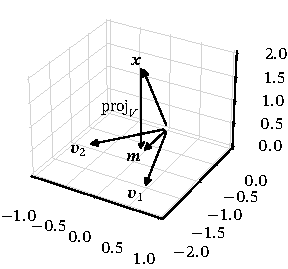
\includegraphics{proj3d.pdf}
  \caption{\(\vect{x}\)の\(V=\spannedby\Set{\vect{v}_1,\vect{v}_2}\)への直交射影\(\vect{m}=\proj_V(\vect{x})\)の模式図.}
\end{figure}

\begin{proposition}{}{}
  \(\numset{K}^n\)の任意の部分空間\(V\)について,写像\(\proj_V\colon\numset{K}^n\to V\)は線型写像である.
\end{proposition}

\begin{proof}
  \(s,t\in\numset{K}\),\(\vect{x},\vect{y}\in\numset{K}^n\)を任意にとり,\(\vect{m}=s\proj_V(\vect{x})+t\proj_V(\vect{y})\)とおく.
  このとき,任意の\(\vect{v}\in V\)に対して\(\innerp{s\vect{x}+t\vect{y}-\vect{m}}{\vect{v}}=s\innerp{\vect{x}-\proj_V(\vect{x})}{\vect{v}}+t\innerp{\vect{y}-\proj_V(\vect{y})}{\vect{v}}=s0+t0=0\)となるので,
  \(\proj_V(s\vect{x}+t\vect{y})=\vect{m}\)である.よって,\(\proj_V\)は線型写像である.
\end{proof}

\subsection{直交補空間}
\begin{definition}{直交補空間}{numerical_perpendicular_complement}\index{ちょっこうほくうかん@直交補空間!かずべくとるくうかんじょうの@数ベクトル空間上の—}\index{\(\pcomp{W}\)}
  \(V\)は\(\numset{K}^n\)の部分空間とする.\(W\)が\(V\)の部分空間なら,集合\(\pcomp{W}=\Set{\vect{x}\in V\given\vect{y}\in W\implies\innerp{\vect{x}}{\vect{y}}=0}\)も\(V\)の部分空間になる.
  \(\pcomp{W}\)を(\(V\)における)\(W\)の\termdef{直交補空間}(orthogonal complement)という.
\end{definition}

\begin{figure}[htbp]
  \centering
  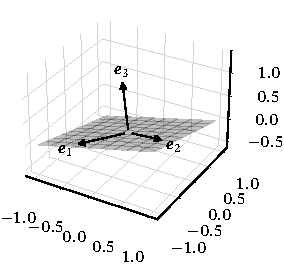
\includegraphics{orthogonal_complement.pdf}
  \caption{2次元部分空間\(W=\spannedby\Set{\vect{e}_1,\vect{e}_2}\)の\(\numset{R}^3\)における直交補空間は,\(\vect{e}_1\)と\(\vect{e}_2\)に直交する\(\zvec\)でないベクトル\(\vect{e}_3\)で生成される直線\(\spannedby\Set{\vect{e}_3}\)である.}
\end{figure}

\begin{proposition}{}{}
  \(V\)は\(\numset{K}^n\)の部分空間で,\(W\)は\(V\)の部分空間とする.このとき\(V=W\oplus\pcomp{W}\)である.
\end{proposition}

\begin{proof}
  \(\vect{x}\in W\cap\pcomp{W}\)なら\(\innerp{\vect{x}}{\vect{x}}=0\)なので\(\vect{x}=\zvec\),よって\(W\cap\pcomp{W}=\Set{\zvec}\)である.
  \cref{proposition:finite_projection}より,各\(\vect{x}\in V\)について\(\vect{x}-\proj_W(\vect{x})\in\pcomp{W}\)であるから,
  \(\vect{x}=\proj_W(\vect{x})+(\vect{x}-\proj_W(\vect{x}))\in W\oplus\pcomp{W}\)である.したがって\(V=W\oplus\pcomp{W}\)である.
\end{proof}

\subsection{スペクトル定理}

\section{最小二乗問題}

\subsection{最小二乗問題}
\subsection{特異値分解}
\subsection{擬似逆行列}

\section{離散フーリエ変換}

\section{多重解像度解析}

\section{主成分分析}
\begin{figure}[htbp]
  \begin{minipage}{\linewidth/2}
    \centering
    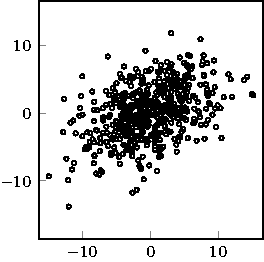
\includegraphics{scatter.pdf}
  \end{minipage}%
  \begin{minipage}{\linewidth/2}
    \centering
    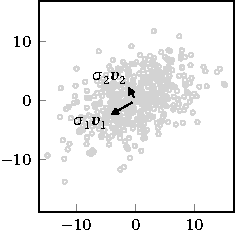
\includegraphics{pca.pdf}
  \end{minipage}
\end{figure}

\begin{subappendices}
\section{低ランク近似}
\end{subappendices}

\section*{演習問題}
\addcontentsline{toc}{section}{演習問題}

\end{document}
